\documentclass[conference]{IEEEtran}

\usepackage{cite}
\usepackage{graphicx}
\usepackage{amsmath}
\usepackage{array}
\usepackage{booktabs}
\usepackage{multirow}
\usepackage{url}
\usepackage{stfloats}

\begin{document}

\title{Content-Based Recommendation System for Flipkart E-Commerce Products}

\author{
\IEEEauthorblockN{O\u{g}uz Alada\u{g}, Ezgi Naz Aydugan, Muhammed Ali Bak\i r}
\IEEEauthorblockA{
Department of Computer Engineering\\
Ankara Bilim University\\
Ankara, Turkiye\\
\{s220205007, s220205031, s220205006\}@ankarabilim.edu.tr}
}

\maketitle

\begin{abstract}
This paper presents a content-based recommendation system developed for Flipkart e-commerce products. The aim of the study is to recommend products that are similar in content to a selected item by using product metadata such as product name, brand, category hierarchy, description, and technical specifications. The selected dataset contains 20,000 product records but does not include user identifiers or explicit user-item interaction histories. Therefore, in accordance with the project guideline for non-interaction datasets, the system is implemented as an item-to-item content-based recommender. During preprocessing, missing values, duplicated products, unstructured specification strings, and noisy text fields were cleaned and normalized. The cleaned product attributes were merged into a unified textual representation and transformed into numerical vectors by using Term Frequency-Inverse Document Frequency (TF-IDF). Cosine similarity was then used to compute similarity between products and generate the top 5 recommendations for a given query item. The model was evaluated on an 80\%-20\% train-test split by defining category-based relevance, where products from the same leaf category were considered relevant and products from the same root category were used as a fallback when necessary. The experimental results yielded a Precision@5 score of 0.9415, a Recall score of 0.1101, and a Mean Average Precision (MAP) score of 0.9343. These findings show that content-based filtering can generate highly relevant top-ranked recommendations for large-scale product catalogs even when collaborative user history is unavailable.
\end{abstract}

\begin{IEEEkeywords}
content-based filtering, recommender systems, TF-IDF, cosine similarity, e-commerce, Flipkart
\end{IEEEkeywords}

\section{Introduction}
Recommendation systems are essential in modern e-commerce platforms because they help users discover relevant items from very large product collections. When thousands of products are available in a single marketplace, manually browsing and comparing all items becomes inefficient. Recommender systems reduce this information overload by ranking and filtering products according to a meaningful relevance criterion. Their use can improve customer satisfaction, support product discovery, and increase platform engagement.

Among the major recommendation paradigms, content-based filtering focuses on the intrinsic properties of items rather than relying solely on the behavior of other users. In this approach, each item is represented by descriptive features such as title, category, attributes, and textual description. Similarity is computed between items in a shared feature space, and recommendations are generated by retrieving items whose content most closely matches the selected query item or a user's previous preferences.

This project develops a content-based recommendation system on a Flipkart product dataset. The dataset is centered on product metadata and contains useful content information such as product name, category tree, brand, retail and discounted price, description, and product specifications. However, the dataset does not provide user IDs, clicks, purchases, ratings linked to users, or any other interaction records that would allow direct personalized recommendation through historical user behavior. For this reason, the project follows the alternative path explicitly permitted in the guideline and implements an item-to-item content-based recommendation model. Instead of recommending products for a known user profile, the system takes a product as input and recommends five new products with similar content characteristics.

The implementation was prepared in both Python script and Jupyter Notebook formats in order to satisfy the project code submission requirement. The Python script performs the complete pipeline automatically, while the notebook version presents the same steps in an interactive and step-by-step structure. Both versions are consistent with the experimental design described in this paper.

The rest of the paper is organized as follows. Section II describes the dataset and its structure. Section III explains the methodology and overall recommendation workflow. Section IV presents the preprocessing operations. Section V explains feature vectorization. Section VI discusses the system design and similarity-based recommendation mechanism. Section VII reports the experimental evaluation results. Section VIII provides discussion and interpretation. Section IX concludes the paper and outlines future work.

\section{Dataset Description}
The dataset used in this study is the uploaded CSV file named \texttt{flipkart\_com-ecommerce\_sample.csv}. It contains product-level records collected from the Flipkart e-commerce platform. The raw dataset includes 20,000 rows and provides several fields that are suitable for content-based recommendation, including \texttt{product\_name}, \texttt{product\_category\_tree}, \texttt{description}, \texttt{brand}, \texttt{retail\_price}, \texttt{discounted\_price}, and \texttt{product\_specifications}. Auxiliary columns such as URLs, images, and crawl timestamps are also present, but they are not central to the recommendation logic.

The most important property of this dataset is that it does not include explicit user-item interactions. Although rating-related columns are present, they are product-side attributes rather than user-linked preference histories, and most entries contain the text ``No rating available.'' As a result, the selected dataset is not suitable for user-based or standard collaborative filtering approaches. Therefore, the recommendation problem was formulated as item-to-item content recommendation.

The dataset also contains common real-world quality issues such as missing brand values, missing descriptions, a small number of missing price values, and duplicate product IDs. These issues make the dataset appropriate for a full preprocessing and feature engineering pipeline. In addition, the dataset has sufficiently rich descriptive content to support a text-driven recommendation approach. Product descriptions and specification fields provide detailed semantic cues, while the category tree offers hierarchical context that is useful both for recommendation and for evaluation.

Table~\ref{tab:dataset_summary} summarizes the cleaned dataset statistics used in the implementation.

\begin{table}[!t]
\caption{Dataset Summary}
\label{tab:dataset_summary}
\centering
\begin{tabular}{|p{0.58\columnwidth}|p{0.22\columnwidth}|}
\hline
\textbf{Metric} & \textbf{Value} \\
\hline
Total raw records & 20,000 \\
\hline
Records after cleaning & 19,998 \\
\hline
Unique products (\texttt{pid}) & 19,998 \\
\hline
Unique brands & 3,500 \\
\hline
Unique root categories & 265 \\
\hline
Missing brand values & 5,864 \\
\hline
Missing description values & 2 \\
\hline
\end{tabular}
\end{table}

To illustrate the structure of the records used during preprocessing and recommendation, Table~\ref{tab:sample_products} provides sample products from the cleaned dataset.

\begin{table}[!t]
\caption{Sample Product Records from the Cleaned Dataset}
\label{tab:sample_products}
\centering
\begin{tabular}{|p{0.28\columnwidth}|p{0.16\columnwidth}|p{0.16\columnwidth}|p{0.18\columnwidth}|}
\hline
\textbf{Product Name} & \textbf{Brand} & \textbf{Root Category} & \textbf{Discounted Price} \\
\hline
Alisha Solid Women's Cycling Shorts & Alisha & clothing & 379 \\
\hline
FabHomeDecor Fabric Double Sofa Bed & FabHomeDecor & furniture & 22646 \\
\hline
AW Bellies & AW & footwear & 499 \\
\hline
Sicons All Purpose Arnica Dog Shampoo & Sicons & pet supplies & 210 \\
\hline
Eternal Gandhi Super Series Crystal Paper Weights & Eternal Gandhi & specialty gifts & 430 \\
\hline
\end{tabular}
\end{table}

\section{Methodology}
The proposed recommendation pipeline follows a standard content-based filtering architecture adapted to the available structure of the dataset. The complete workflow consists of the following stages:

\begin{enumerate}
\item loading the raw CSV dataset,
\item cleaning missing values and duplicate products,
\item extracting and normalizing relevant content features,
\item combining textual and categorical content into a single representation,
\item transforming the combined text into TF-IDF feature vectors,
\item computing cosine similarity between product vectors,
\item returning the top 5 most similar items for a selected query product, and
\item evaluating the ranking performance with Precision@5, Recall, and MAP.
\end{enumerate}

Since user interaction data is absent, a direct personalized recommendation protocol cannot be applied. The project guideline explicitly allows an item-based recommendation design in such cases. Therefore, the system takes a selected item as the query, compares it against all candidate items in the training set, and retrieves five products with the highest similarity scores after excluding the identical product itself.

Evaluation also required a careful adaptation. In collaborative recommendation problems, relevance is typically defined through historical user feedback such as clicks, ratings, or purchases. Here, a category-based relevance strategy was defined. For each test item, products from the same leaf category in the training set were treated as relevant. If the number of items in the same leaf category was insufficient, the root category was used as a fallback. This strategy provides a consistent way to measure whether the recommended items are semantically aligned with the query item.

\subsection{Implementation Workflow}
The project code directly follows the methodology above. The Python script first loads the CSV file into a dataframe and examines the available columns and missing values. Then it removes duplicate identifiers, fills missing content fields, parses category hierarchy information, and constructs cleaned textual features. After preprocessing, the data is divided into 80\% training and 20\% testing partitions using a random but reproducible split.

The TF-IDF vectorizer is fitted only on the training set, which prevents leakage from the test set into the learned vocabulary space. Next, the same vectorizer is applied to the test set and to individual query products. Recommendations are generated by computing cosine similarity between a query vector and all candidate vectors from the training pool, sorting the scores, filtering out the identical item, and returning the top 5 results.

Finally, the same ranking process is repeated for all test products to compute aggregate evaluation metrics. The implementation also exports CSV tables and PNG figures used in the report, ensuring that the code and the paper remain fully consistent.

\section{Data Preprocessing}
Data preprocessing is a critical step in content-based recommendation because the quality of recommendations depends directly on the quality and consistency of item features. The raw Flipkart dataset contains both structured and unstructured fields, and several preprocessing operations were applied before model training.

First, duplicate records were removed. The implementation eliminated duplicate \texttt{uniq\_id} entries and repeated \texttt{pid} values while keeping the first valid product instance. This ensured that the recommendation space was composed of unique items only.

Second, missing values were handled. Missing \texttt{brand} values were replaced with the token \texttt{unknown} so that the feature space preserved a consistent brand field for every product. Missing values in \texttt{description} and \texttt{product\_specifications} were replaced with empty strings. Retail and discounted prices were converted to numeric data types and any missing numeric entries were filled with median values to avoid null values in descriptive tables.

Third, the hierarchical category field was parsed. The original \texttt{product\_category\_tree} column contains nested category paths. This field was split to derive both the root category and the leaf category. The root category provides a broad semantic grouping such as \texttt{clothing} or \texttt{furniture}, whereas the leaf category captures more specific product identity.

Fourth, textual normalization was applied to all content fields used in the recommender. The operations included lowercasing, ASCII normalization, URL removal, punctuation cleaning, stopword removal, and whitespace normalization. Product specifications were originally stored in a noisy semi-structured text format and were simplified into plain text so that relevant attribute words could still contribute to similarity.

Finally, the cleaned product name, brand, category path, description, and specifications were concatenated into a single combined text field. This unified representation became the basis for feature vectorization.

\subsection{Why Preprocessing Was Important}
The preprocessing stage directly affects both the quality of similarity computation and the validity of the final evaluation. Without normalization, the same concept may appear in multiple forms because of punctuation, uppercase-lowercase differences, or noisy formatting. Without duplicate removal, the model may recommend repeated products, which would artificially inflate similarity results. Without parsing the category hierarchy, the system would not be able to construct a reasonable relevance definition for evaluation in a non-interaction setting. For these reasons, preprocessing is not merely a cleaning step but a core design component of the recommender.

\begin{figure*}[!t]
\centering
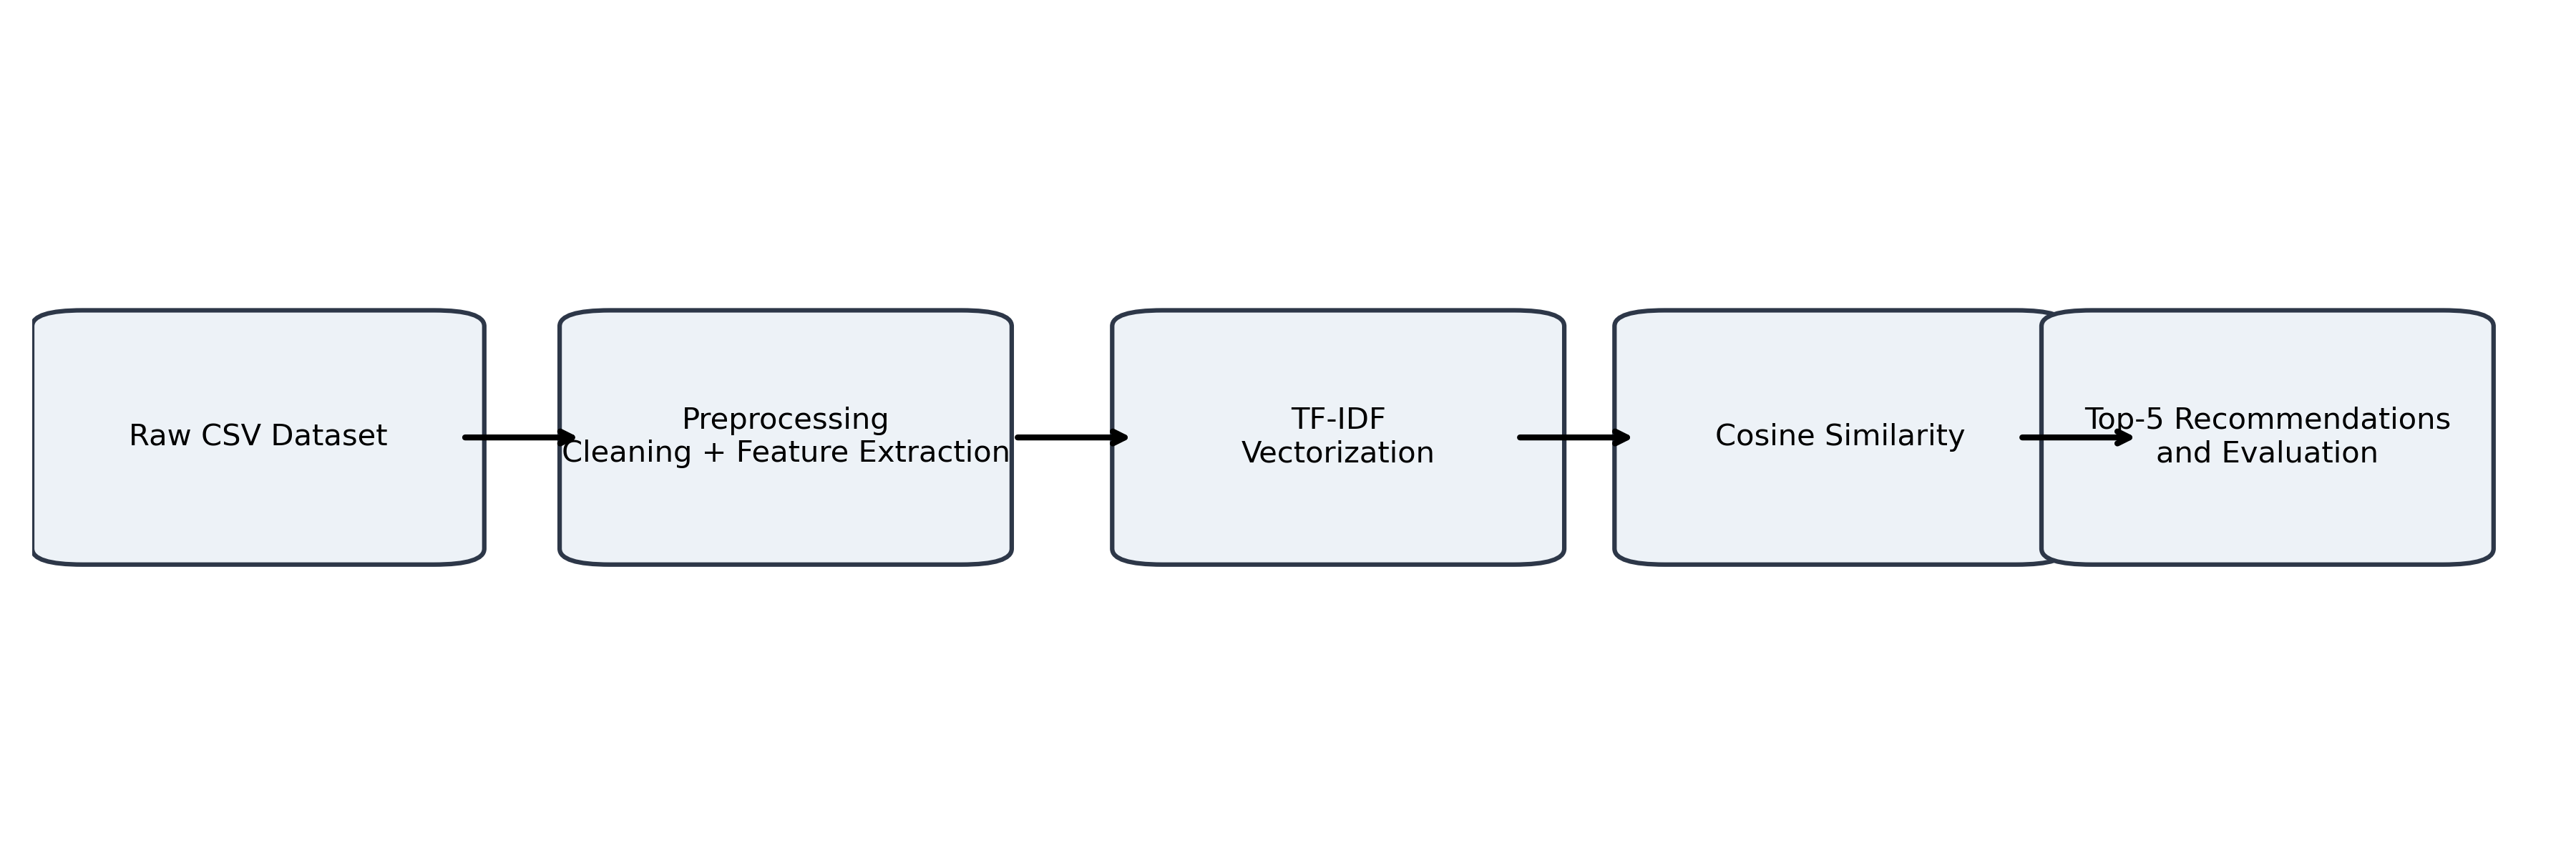
\includegraphics[width=0.90\textwidth]{outputs/figures/recommendation_pipeline.png}
\caption{System architecture and content-based recommendation pipeline.}
\label{fig:pipeline}
\end{figure*}

\section{Feature Vectorization}
After preprocessing, each product must be represented numerically so that similarity can be computed mathematically. In this project, feature vectorization was performed using Term Frequency-Inverse Document Frequency (TF-IDF), which is one of the most widely used methods for representing text in information retrieval and recommendation problems.

The combined text field for each product includes the cleaned product name, brand, category path, description, and product specifications. A TF-IDF vectorizer was fitted on the training set using unigram and bigram features. This setting allows the model to capture both individual terms and short word combinations that are highly informative in e-commerce descriptions, such as product materials, styles, dimensions, categories, and brand-specific terminology.

TF-IDF assigns higher weights to terms that appear frequently in a particular item but are less common across the full corpus. This helps emphasize discriminative product terms while reducing the influence of generic words. Compared with simple count vectors, TF-IDF generally produces a more informative similarity space for text-rich product catalogs.

The resulting sparse vectors represent each product in a high-dimensional semantic feature space. Once this representation is created, the recommender can compare products by computing vector similarity scores.

\subsection{Feature Configuration}
The implementation uses a TF-IDF vectorizer configured with unigrams and bigrams and a bounded vocabulary size. This choice offers a practical balance between expressiveness and computational efficiency. Unigrams capture single descriptive words such as material, category, and color terms, while bigrams capture short expressions such as ``sofa bed,'' ``cycling shorts,'' and ``patent leather.'' These phrase-level patterns are useful in product recommendation because they often carry stronger semantic meaning than isolated tokens.

\subsection{Why TF-IDF Was Chosen}
TF-IDF was preferred over pure one-hot encoding and simple count-based text models because the dataset contains long and descriptive textual fields. One-hot encoding is appropriate for compact categorical variables but is insufficient for unstructured descriptions and specifications. TF-IDF is better suited for this case because it naturally scales to textual content and emphasizes distinguishing terms that help identify item similarity.

\section{System Design}
The system design consists of five tightly connected modules: data loading, preprocessing, vectorization, similarity computation, and recommendation generation. The end-to-end architecture is shown in Fig.~\ref{fig:pipeline}. The implementation was developed in Python and uses common data science libraries, including \texttt{pandas}, \texttt{scikit-learn}, \texttt{numpy}, and \texttt{matplotlib}.

\subsection{Similarity Computation}
Product similarity was computed with cosine similarity, which is a standard metric for TF-IDF vectors. Given two product vectors $A$ and $B$, cosine similarity is defined as
\begin{equation}
\text{CosineSimilarity}(A, B) = \frac{A \cdot B}{\|A\| \|B\|}.
\end{equation}

This metric measures the angle between two vectors rather than the raw magnitude difference. As a result, it is well suited for sparse text representations because it focuses on the overlap of important terms. Two products with highly similar content fields obtain a similarity score close to 1, while semantically unrelated items obtain scores closer to 0.

In the implementation, cosine similarity is applied between a query vector and the TF-IDF matrix of candidate items. This produces a ranked similarity score for every product in the training set. Because the vectors are sparse and high dimensional, cosine similarity provides an efficient and interpretable measure of semantic proximity without requiring more complex latent-factor or neural methods.

\subsection{Recommendation Generation}
The recommendation process begins with a selected query product. The item is transformed into the same TF-IDF feature space as the training items. Next, cosine similarity is computed between the query vector and all candidate item vectors in the training set. The products are then ranked in descending order according to similarity score. The identical product is removed from the candidate list, and the top 5 highest-ranked items are returned as recommendations.

Because the dataset lacks user histories, this approach represents the best content-driven interpretation of the instructor requirements. It still satisfies the requirement to output five recommendations, but the recommendations are generated for a given item rather than for a user profile.

In practice, the model tends to retrieve items from the same product family, style, or usage context because the combined feature field includes multiple complementary attributes. For example, apparel items usually retrieve other products with similar fabric, style, and category phrases, while furniture products tend to match on structural keywords and category hierarchy.

Table~\ref{tab:example_recs} shows a sample recommendation output from the implemented system.

\begin{table}[!t]
\caption{Example Top-5 Recommendations for a Query Product}
\label{tab:example_recs}
\centering
\begin{tabular}{|p{0.38\columnwidth}|p{0.18\columnwidth}|p{0.14\columnwidth}|}
\hline
\textbf{Recommended Product} & \textbf{Brand} & \textbf{Similarity} \\
\hline
Cayman Full Sleeve Solid Men's Sweatshirt & unknown & 0.3318 \\
\hline
Ashdan Sleeveless Solid Men's Sweatshirt & Ashdan & 0.3303 \\
\hline
Absurd Full Sleeve Solid Men's Reversible Sweatshirt & unknown & 0.3220 \\
\hline
People Full Sleeve Solid Men's Sweatshirt & unknown & 0.3207 \\
\hline
Fila Full Sleeve Solid Men's Reversible Sweatshirt & unknown & 0.3189 \\
\hline
\end{tabular}
\end{table}

\section{Experimental Results and Evaluation}
To evaluate the model, the cleaned dataset was divided into 80\% training items and 20\% testing items. The TF-IDF vectorizer was fitted only on the training data, and the test items were transformed into the learned feature space. For every test item, the recommender returned the top 5 most similar products from the training set.

Since no user feedback is available, evaluation used the category-based relevance strategy described earlier. A recommended item was treated as relevant if it belonged to the same leaf category as the query item, with root category used as a fallback when required. This relevance definition made it possible to compute ranking-based information retrieval metrics on the recommendation output.

\subsection{Metric Definitions}
Let $k=5$ denote the recommendation list length. Precision@5 measures the fraction of the five recommended products that are relevant. Recall measures how many of all relevant products in the candidate pool were successfully retrieved among these top five results. Mean Average Precision (MAP) measures ranking quality more strictly because it rewards systems that place relevant items earlier in the ranked list instead of merely including them somewhere in the top recommendations.

These metrics were selected because they are standard for recommendation and ranking tasks. Precision@5 is especially appropriate here because the project requirement explicitly asks for five recommendations. MAP complements precision by evaluating the internal ordering of the recommendation list, while recall shows the natural limitation of returning a very small ranked set from potentially large relevant categories.

The required evaluation metrics are defined as follows:
\begin{itemize}
\item \textbf{Precision@5}: the proportion of relevant items among the top 5 recommended products.
\item \textbf{Recall}: the proportion of all relevant candidate items that appear in the recommended list.
\item \textbf{MAP}: the mean of average precision values computed over all evaluated test products.
\end{itemize}

Table~\ref{tab:eval_results} presents the aggregated evaluation results produced by the implementation.

\begin{table}[!t]
\caption{Performance Evaluation Results}
\label{tab:eval_results}
\centering
\begin{tabular}{|p{0.32\columnwidth}|p{0.22\columnwidth}|}
\hline
\textbf{Metric} & \textbf{Score} \\
\hline
Precision@5 & 0.9415 \\
\hline
Recall & 0.1101 \\
\hline
MAP & 0.9343 \\
\hline
Evaluated Items & 3961 \\
\hline
\end{tabular}
\end{table}

The scores indicate that the proposed recommender is highly effective at placing category-consistent and semantically similar products near the top of the ranking. The very high Precision@5 and MAP values show that the first five recommended products are usually strongly aligned with the content of the query item. The lower recall is expected in this setup because many categories contain a large number of relevant products, but only five recommendations are returned. Therefore, the system is optimized for accurate top-ranked retrieval rather than for covering the full set of relevant items.

Another important interpretation is that the metric profile matches the intended usage scenario of the system. In a realistic e-commerce interface, users usually inspect only a small number of top recommendations displayed in product detail pages or recommendation widgets. For such short lists, high precision at top ranks is often more valuable than maximizing global recall. The results therefore suggest that the proposed model is appropriate for practical item-similarity recommendation tasks.

To provide visual support for the experimental section, Fig.~\ref{fig:categories} shows the category distribution of the most frequent root categories, and Fig.~\ref{fig:metrics} presents the final evaluation metric comparison.

\begin{figure*}[!t]
\centering
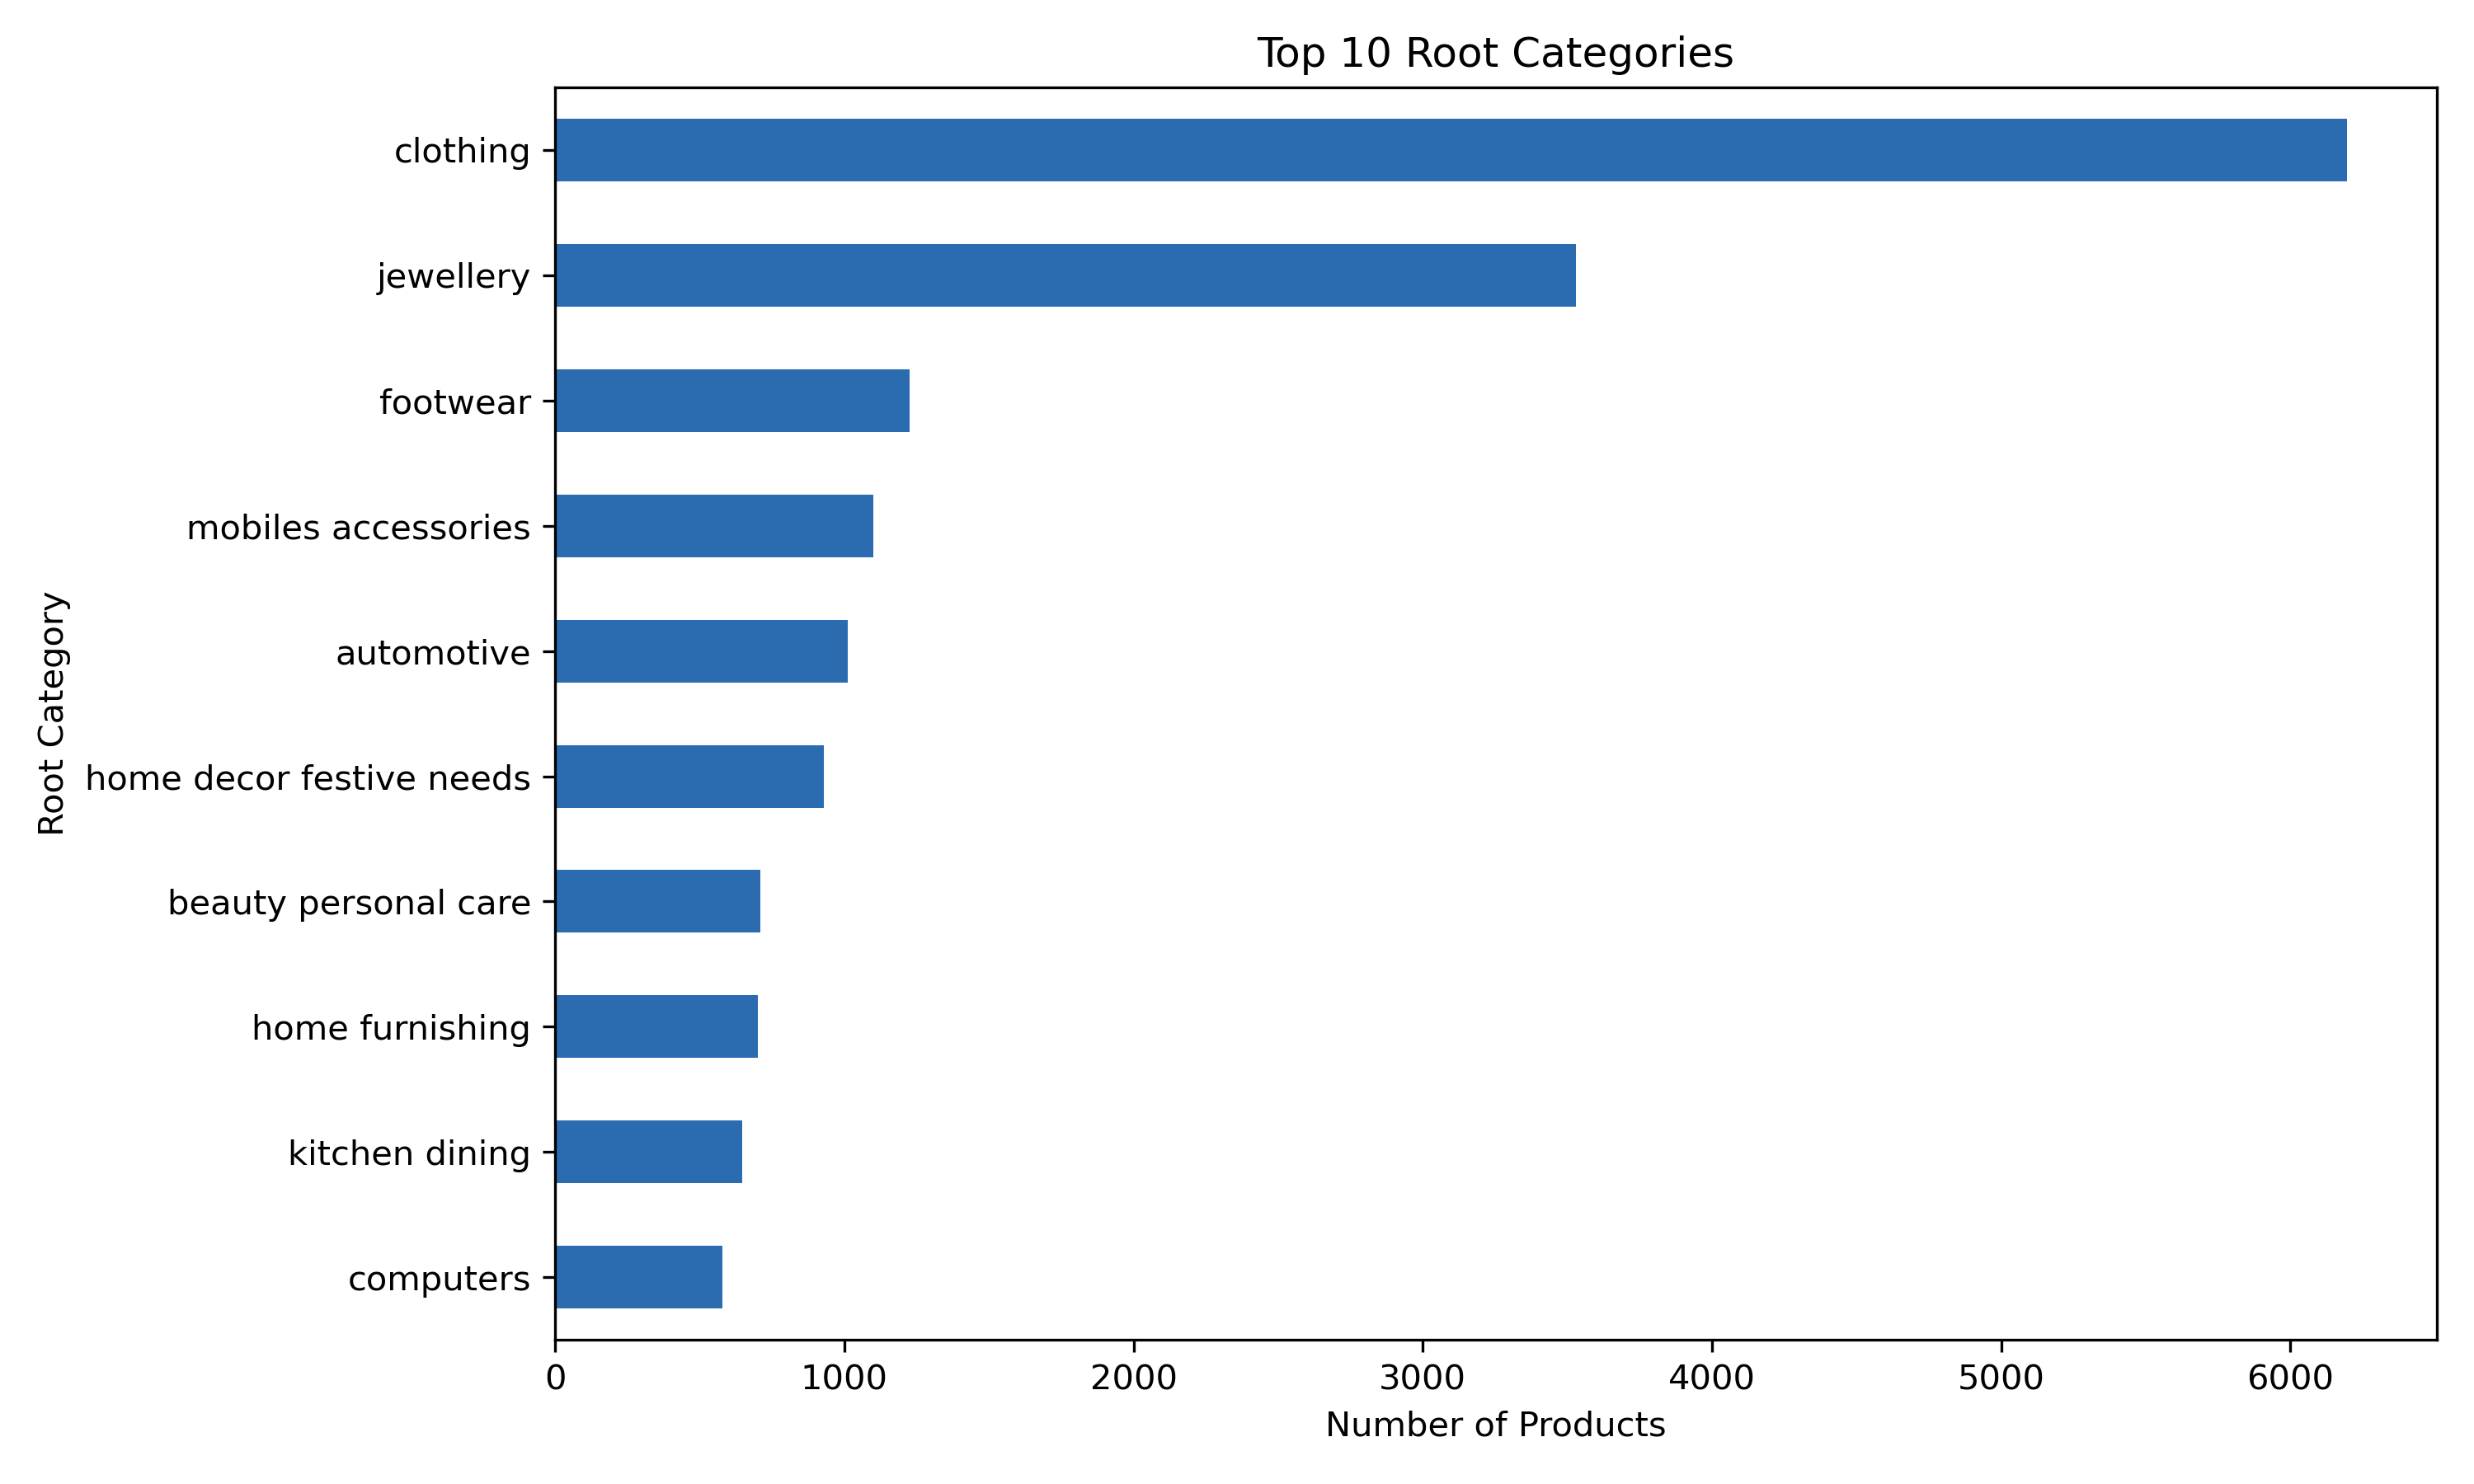
\includegraphics[width=0.88\textwidth]{outputs/figures/top_categories.png}
\caption{Top 10 root categories in the cleaned Flipkart dataset.}
\label{fig:categories}
\end{figure*}

\begin{figure*}[!t]
\centering
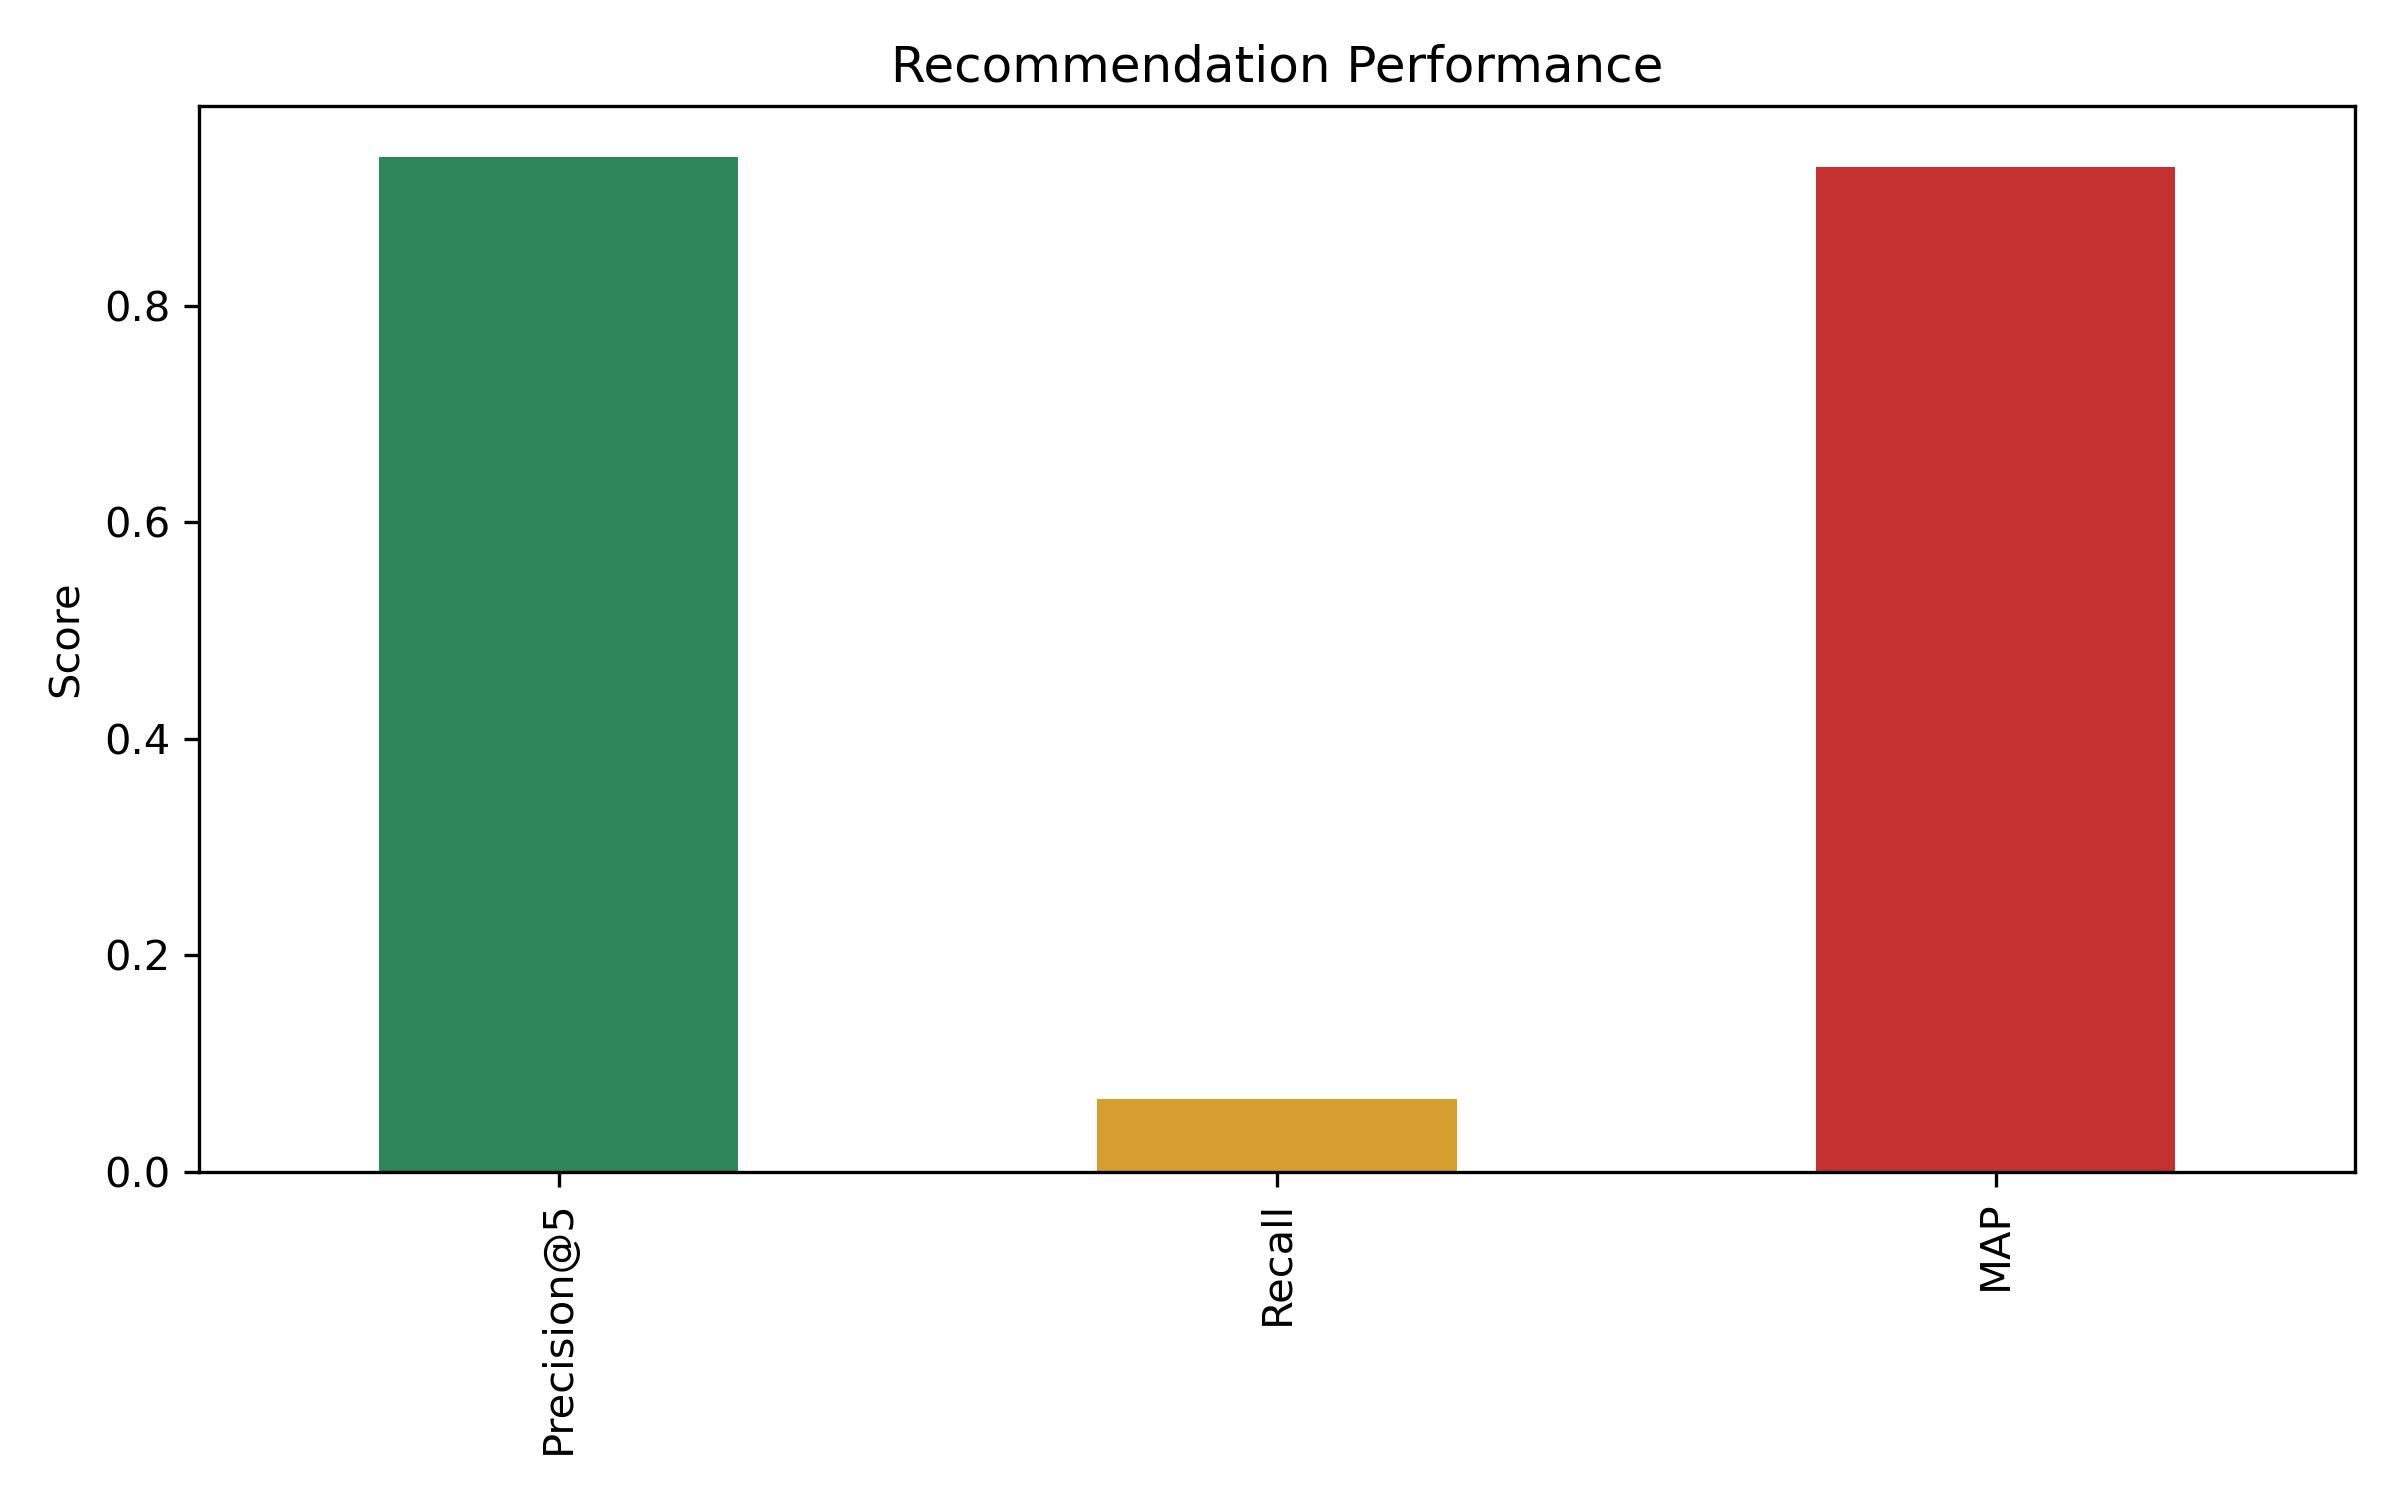
\includegraphics[width=0.84\textwidth]{outputs/figures/evaluation_metrics.png}
\caption{Comparison of Precision@5, Recall, and MAP scores.}
\label{fig:metrics}
\end{figure*}

\section{Discussion}
The experimental findings demonstrate that content-based filtering can be highly effective when product metadata is rich and descriptive. In this dataset, the combination of product title, brand, hierarchical category information, description text, and specifications creates a strong semantic representation for matching related products. The high Precision@5 and MAP values confirm that the model ranks highly relevant items at the top of the recommendation list.

At the same time, several limitations must be acknowledged. First, the system is not personalized at the user level because the dataset does not include user histories. Second, the relevance definition is category based rather than behavior based, which means it is a reasonable proxy but not a substitute for true user preference signals. Third, some category names and specification strings in the dataset are noisy or truncated, which can reduce representation quality for certain products.

Another limitation is that TF-IDF is fundamentally a lexical representation. If two products are semantically similar but described with substantially different wording, the similarity score may not fully reflect that relationship. In addition, the current system does not incorporate visual product features, review text, or session behavior, all of which could further improve recommendation quality in a richer production system.

Despite these limitations, the model remains fully consistent with the instructor guideline. The guideline explicitly states that when user interactions are not available, students should implement an item-to-item recommendation system and define an appropriate evaluation strategy. The proposed approach satisfies both conditions in a technically valid and reproducible way.

From a project perspective, the implemented system still provides a complete demonstration of content-based recommendation methodology. It covers dataset understanding, preprocessing, feature engineering, vectorization, similarity measurement, recommendation ranking, and evaluation. For this reason, the work satisfies both the technical objective of the course project and the reporting requirements expected in an IEEE-style paper.

\section{Conclusion and Future Work}
This paper presented a complete content-based recommendation system for Flipkart e-commerce products. Because the dataset did not contain user-item interaction records, the recommendation problem was formulated as item-to-item recommendation using product content features. A full pipeline was developed, including preprocessing, category parsing, text normalization, TF-IDF vectorization, cosine similarity computation, top-5 recommendation generation, and evaluation with Precision@5, Recall, and MAP.

The obtained results show that the proposed method is effective at retrieving highly relevant products in the top positions of the recommendation list. This confirms that content-based filtering remains a practical solution when interaction-based collaborative filtering cannot be applied.

Future work can improve the system in several directions. Pre-trained word embeddings or transformer-based sentence embeddings may capture richer semantics than TF-IDF. Product images could be incorporated to build a multimodal recommender. Structured parsing of product specifications could also be improved so that material, size, color, and technical attributes are treated as separate engineered features instead of generic text. If user histories become available in future datasets, a hybrid system that combines collaborative filtering and content-based filtering can also be developed. In addition, future studies can compare TF-IDF against transformer-based embedding models and evaluate not only relevance but also recommendation diversity and novelty.

\section*{Acknowledgment}
This project was developed as part of a course assignment in recommendation systems and data mining. The authors would like to thank the course instructor for the guideline, evaluation criteria, and dataset selection process.

\begin{thebibliography}{99}

\bibitem{ricci}
F. Ricci, L. Rokach, and B. Shapira, \emph{Recommender Systems Handbook}. Boston, MA, USA: Springer, 2015.

\bibitem{manning}
C. D. Manning, P. Raghavan, and H. Sch\"utze, \emph{Introduction to Information Retrieval}. Cambridge, U.K.: Cambridge University Press, 2008.

\bibitem{leskovec}
J. Leskovec, A. Rajaraman, and J. D. Ullman, \emph{Mining of Massive Datasets}, 3rd ed. Cambridge, U.K.: Cambridge University Press, 2020.

\bibitem{salton}
G. Salton and M. J. McGill, \emph{Introduction to Modern Information Retrieval}. New York, NY, USA: McGraw-Hill, 1983.

\bibitem{lops}
P. Lops, M. de Gemmis, and G. Semeraro, ``Content-based recommender systems: State of the art and trends,'' in \emph{Recommender Systems Handbook}, F. Ricci, L. Rokach, B. Shapira, and P. B. Kantor, Eds. Boston, MA, USA: Springer, 2011, pp. 73--105.

\bibitem{aggarwal}
C. C. Aggarwal, \emph{Recommender Systems: The Textbook}. Cham, Switzerland: Springer, 2016.

\end{thebibliography}

\end{document}
